\ifx \globalmark \undefined %% This is default.
	\documentclass[twoside,openright,11pt,a4paper]{report}

%\compiler avec xelatex
%\usepackage[applemac]{inputenc}
\usepackage[T1]{fontenc}
\usepackage[utf8]{inputenc} %latin1 est possible
%\usepackage[latin1]{inputenc} %latin1 est possible
\usepackage[UKenglish]{babel}
\usepackage{lettrine}

%\usepackage[text={13cm,20cm},centering]{geometry}
\usepackage [squaren, Gray, mediumqspace]{SIunits}
\usepackage [top=2cm, bottom=2cm, left=2cm, right=2cm ]{geometry}

\renewcommand{\familydefault}{cmss}
\addto\captionsenglish{ \renewcommand\chaptername{Solutions of Chapte}}

\usepackage{graphicx}
\usepackage{amsmath}
\usepackage{amsfonts}
\usepackage{amssymb}
\usepackage{amsthm}
\usepackage{bm}
\usepackage{color}

\newcommand{\real}{\mathbb{R}}
\newcommand{\mb}{\mathbf}
\newcommand{\bos}{\boldsymbol}

\def \RR {I \! \! R}

\newcommand{\e}{\begin{equation}}  
\newcommand{\ee}{\end{equation}}
\newcommand{\eqn}{\begin{eqnarray}} 
\newcommand{\eeqn}{\end{eqnarray}} 
\newcommand{\eqnn}{\begin{eqnarray*}} 
\newcommand{\eeqnn}{\end{eqnarray*}} 

\newcommand{\bpm}{\begin{pmatrix}}
\newcommand{\epm}{\end{pmatrix}}

%\newcommand{\{\c c}}{\c c}

\newcommand{\bma}{\left(\begin{array}}
\newcommand{\ema}{\end{array}\right)} 
\newcommand{\hh}{\hspace{2mm}}
\newcommand{\hd}{\hspace{5mm}}
\newcommand{\hu}{\hspace{1cm}}
\newcommand{\vv}{\vspace{2mm}}
\newcommand{\vd}{\vspace{5mm}}
\newcommand{\vm}{\vspace{-2mm}}
\newcommand{\teq}{\triangleq}
%\newcommand{\qedb}{\,$\Box$}
\newcommand{\blanc}{$\left. \right.$}
\newcommand{\frts}[2]%
         {\frac{{\textstyle #1}}{{\textstyle #2}}}

\newcommand{\bindex}[3]%
{
\renewcommand{\arraystretch}{0.5}
\begin{array}[t]{c}
#1\\
{\scriptstyle #2}\\
{\scriptstyle #3}
\end{array}
\renewcommand{\arraystretch}{1}
}

\theoremstyle{definition}
\newtheorem{exemple}{{\bf Exemple}}[chapter]
\newtheorem{theoreme}[exemple]{{\bf Th{é}or{è}me}}
\newtheorem{propriete}[exemple]{{\bf Propri{é}t{é}}}
\newtheorem{definition}[exemple]{{\bf D{é}finition}}
\newtheorem{remarque}[exemple]{{\bf Remarque}}
\newtheorem{remarques}[exemple]{{\bf Remarques}}
\newtheorem{lemme}[exemple]{{\bf Lemme}}
\newtheorem{hypothese}[exemple]{{\bf Hypoth{è}se}}
\newtheorem{exercice}{{\bf Exercice}}[chapter]

\newcommand{\xqedhere}[2]{%
 \rlap{\hbox to#1{\hfil\llap{\ensuremath{#2}}}}}

\newcommand{\xqed}[1]{%
 \leavevmode\unskip\penalty9999 \hbox{}\nobreak\hfill
 \quad\hbox{\ensuremath{#1}}}

\newcommand{\gf}{\fg\,\,}

\newcommand{\cata}[1] %
     {\renewcommand{\arraystretch}{0.5}
     \begin{array}[t]{c} \longrightarrow \\ {#1} \end{array}
     \renewcommand{\arraystretch}{1}}

\usepackage[isu]{caption}
%\usepackage[font=small,format=plain,labelfont=bf,up,textfont=it,up]{caption}
\setlength{\captionmargin}{60pt}

\newcommand{\cqfd}
{%
\mbox{}%
\nolinebreak%
\hfill%
\rule{2mm}{2mm}%
\medbreak%
\par%
}

\pagestyle{headings}

\renewcommand{\sectionmark}[1]{%
\markright{\thesection.\ #1}{}}

\renewcommand{\chaptermark}[1]{%
\markboth{\chaptername\ \thechapter.\ #1}{}}

\makeatletter 
\def\@seccntformat#1{\csname the#1\endcsname.\;} 
\makeatother

\title{ {\Huge {\textbf{Modélisation et analyse  \\ \vspace{4mm} des systèmes dynamiques }}} \\ \vspace{4cm} G. Bastin}

%\title{ {\Huge {\textbf{Modelisation et analyse  \\ \vspace{4mm} des systemes dynamiques }}} \\ \vspace{4cm} G. Bastin}


\date{\today}
	\begin{document} %% Crashes if put after (one of the many mysteries of LaTeX?).
\else 
	\documentclass{standalone}
	\begin{document}
\fi

\graphicspath{ {Chapitre4/images/} }

\setcounter{chapter}{3}
\chapter{Compartment systems}
\chaptermark{Compartment system}\label{syscompart}

\lettrine[lines=1]{\bf T}{}he notion of compartment system is used to specify a wide set of systems for which the dynamic can be described  by balanced equations.
It is used in many engineering fields (such as chemistry engineering, biomedical engineering or ecology), in economy and social sciences as well. 

\section{Definitions and notations}
A compartment is a conceptual tank or box for which the content (matter, energy, money, population...) can be quantified.
The symbolic notation used is depicted at figure \ref{fig:compartiment} 
where $q_{in}$ and $q_{out}$ are respectively the filling and emptying flows 
of the compartment expressed in quantity of content by time unit.
These flows are always {\em positive}, by convention.

\begin{figure}[ht]
\begin{center}
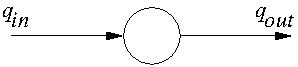
\includegraphics{images/compartiment}
\caption{Symbolic representation of the compartment.}
\label{fig:compartiment}
\end{center}
\end{figure}

A compartment system is made of one {\em network} of compartments 
interconnected and labelled $1$ through $n$.
To be clear, an example of system made of $3$ compartments is shown
at figure \ref{fig:exemplecomp}. The arrows specify the flows of content
exchanged by the the compartment in the network and with outside of 
the system.

\begin{figure}[ht]
\begin{center}
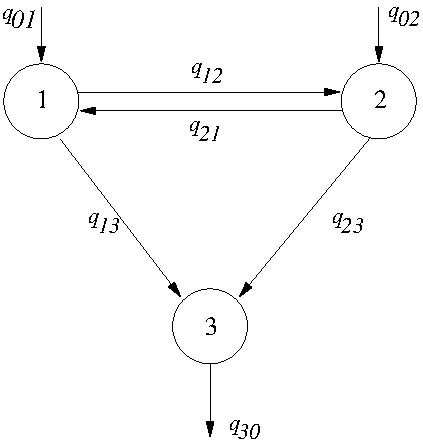
\includegraphics[width=5cm]{images/exemplecomp}
\caption{An example of a compartment system graph.}
\label{fig:exemplecomp}
\end{center} 
\end{figure}

In general, a compartment system is represented by an {\em oriented graph} 
whose nodes correspond to compartments and arcs to flows. 
The following notations are introduced~:
\begin{description}
\item $x_i$ is the quantity of content in the compartment of indices $i$,
$(i = 1, ... ,n)$. This quantity is always {\em positive}. Using a slight abuse of terms,
$x_i$ is used to depict the {\em level} of matter in the compartment $i$.
\item $q_{ij}$ specify the flow flowing from compartment $i$ towards the  
compartment $j$, $(i = 1, ... ,n ; j = 1, ... ,n)$. As mentioned above, it is a
variable which is always {\em positive} by convention.
\end{description}

\begin{definition}{\bf \em Open or close system}
A system is {\bf open} when there exists a possibility to exchange matter
with outside the system.
In this case :  
\begin{description}
\item $q_{io}$ specify the flow from  compartment $i$ towards the outside
\item $q_{oi}$ specify the flow from the outside towards the compartment $i$
\end{description}
Otherwise, the system is said to be {\bf close} : $q_{io} = 
q_{oi} = 0$ for all $i$. \qed
\end{definition}

\begin{definition}{\bf \em System connected to entrances and exits}

A compartment $i$ is {\it connected to an exit} if there is a path $i \rightarrow j \rightarrow k \rightarrow \dots \rightarrow \ell$ from this compartment ending in a compartment $\ell$ from which there is an outgoing flow  $q_{\ell o}$. The system is {\it completely connected to the exits} (CCO) if each and every compartment is connected to an exit.

A compartment $\ell$ is {\it connected to an entry} if there is a path $i \rightarrow j \rightarrow k \rightarrow \dots \rightarrow \ell$ ending in this compartment and coming from a compartment $i$ in which there is an entering flow $q_{oi}$. The system is {\it completely connected to the entries} (CCI) if every compartment is connected to an entry. \qed 
\end{definition}


\section{State model}
\markboth{ {\bf \hspace*{5mm}Chapter 4 }\hfill Compartment system} {{ \bf Sec. \thesection} \hfill
State model \hspace*{5mm}}

The balanced equation of every compartment (also called continuity equation)
\eqnn
\dot{x_i} = \sum_{j=0}^n q_{ji}(t) - \sum_{j=0}^n q_{ij}(t) \hspace{1cm} i=1,...,n
\label{bilan}
\eeqnn
is the basic statement to establish the state model of a compartment system.
This equation tells us that the variation, per unit of time, of the 
quantity contained in a compartment is the difference between the 
sum of the entering flows (or debits) and the sum of the outgoing flows (or debits). 
In practice, of course, the flows wich are structurely null are not explicitly in the equation  
(\eqref{bilan}).

Computing the equations of the sate model of a compartment system required two 
fundamental aspects. 

First of all, the structure of the graph related to the system determines the 
number and the structure of the balanced equations (\eqref{bilan}) ; the variables $x_i$ are
the state variables whereas the order of the model is the number $n$ of  
compartments.

To complete the state model, the flows should be specified in terms of the 
state variables and input variables : 
\eqnn
q_{ij}(x,u)
\eeqnn
where $x$ et $u$ are, as usual, the vector of state and entries. 
This modelling is the point of the next section.

The general form of the state equations of a compartment system is the 
following :  
\eqnn
\dot{x_i} = \sum_{j=0}^n q_{ji}(x,u) - \sum_{j=0}^n q_{ij}(x,u) \hspace{1cm} i=1,...,n \label{eqetcomp}
\eeqnn
In this model, the physical meaning of the state variables $x_i$ is obvious : these are
the quantities contained in each compartment. But, the input variables $u$ can be 
of different nature, depending on the applications, as the next examples will show.

If the {\em flows vector} $q(x,u)$ is defined as containing, in an arbitrary order, all the
flows $q_{ij}(x,u)$ which are not structurally null, then the sate model (\eqref{eqetcomp}) 
can also be written in a more compact matrix form :
\eqn
\dot{x} = Lq(x,u) \label{modetcomp}
\eeqn
where $L$ is the incident matrix of the oriented graph, whose  
coefficents all belong to 
$(-1,0,1)$, which is ?????.

\begin{exemple}
For the system depicted at figure \ref{fig:exemplecomp}, the
state model is written as :
\eqnn
\dot{x_1} &=& q_{01}(x,u) - q_{12}(x,u) - q_{13}(x,u) + q_{21}(x,u) \\
\dot{x_2} &=& q_{02}(x,u) + q_{12}(x,u) - q_{21}(x,u) - q_{23}(x,u) \\
\dot{x_3} &=& q_{13}(x,u) + q_{23}(x,u) - q_{30}(x,u)
\eeqnn
If the flows vector is defined as :
\eqnn
q(x,u) \triangleq \bma{c} q_{01}(x,u) \\ q_{02}(x,u) \\ q_{12}(x,u) \\
q_{13}(x,u) \\ q_{21}(x,u) \\ q_{23}(x,u) \\ q_{30}(x,u) \ema
\eeqnn
the state model is written in a matrix format (\eqref{modetcomp}) with  
the matrix $L$ :
\eqnn
L \triangleq \bma{ccccccc} 1 & 0 & -1 & -1 & 1 & 0 & 0 \\
0 & 1 & 1 & 0 & -1 & -1 & 0 \\
0 & 0 & 0 & 1 & 0 & 1 & -1 \ema.
\eeqnn
\qed
\end{exemple}

\section{Modelling of the flows}

Depending on the applications, the functions $q_{ij}(x,u)$ depicting the flows can take different types of
forms. However, they must be defined in a way which guarantees the compartment system to be a {\em positive system}, that is a system for which every state variable remains positive along the trajectories. 
It is a likelihood guarantee of the model, because the state variables represent measures which do not have a 
physical meaning if they are negative.

\begin{definition} \label{vecpositif} {\bf \em Positive vector and positive orthant}

A vector $x = (x_1, \ldots , x_n)^T$ is positive (notation
$x \geq 0$) if each of its component is a positive real number~:
$x_i \geq 0$ for all $i$.

The positive orthant of dimension $n$ (written $\RR_+^n$) is the set of all positive vectors of dimension $n$. \qed
\end{definition}

\begin{definition}{\bf \em Positive system}

A dynamical system $\dot x=f(x,u)$ is a positive system if, for every admissible input $u(t)$, its 
state is confined in the positive orthant when the initial state is positive~:
\eqnn
x(t_0) \in \real_+^n \text{ et } u(t) \in {\cal U}  \Longrightarrow x(t)
\in \real_+^n  \hh \forall t \geq t_0. \qed
\eeqnn
\end{definition}

The following theorem gives a sufficient condition which can be easily used to 
check that a system is positive.

\begin{theoreme} 
A dynamical system $\dot x=f(x,u)$ is a positive system if $f(x,u)$ is differentiable and if 
\eqnn
x \in \real_+^n \;\;\;\; \mbox{et} \;\;\;\; x_i = 0 \;\; \Longrightarrow \;\; \dot x_i \geq 0 \;\;\;\; \forall i. \qed
\eeqnn
\end{theoreme}
To ensure that a compartment system is a positive system, let's impose the following conditions on the 
flows functions $q_{ij}(x,u)$~:
\begin{itemize}
\item[C1.]  The functions $q_{ij}(x,u)$ are positive functions of their arguments on their definition domain~:
\eqnn
q_{ij}(x,u) : \real^n_+ \times \real^m \rightarrow \real_+
\eeqnn 
\item[C2.] The functions $q_{ij}(x,u)$ are continuous and differentiable functions of their arguments on their
definition domain.
\item[C3.]  As there cannot be an outgoing flow from an empty compartment, the 
functions $q_{ij}(x,u)$ verify the condition~:
\eqnn
x_i = 0 \;\; \Rightarrow \;\; q_{ij}(x,u) = 0
\eeqnn
\end{itemize}
\begin{theoreme} 

Under conditions C1, C2, C3, a dynamical compartment system $\dot x = Lq(x,u)$
is a positive system.
\cqfd
\end{theoreme}

\begin{exemple}\label{systhyd}{\bf \em Hydraulic system}

Let's consider an hydraulic system made of a set of 
tanks located at different elevations and whose the liquid content  
flows \og as waterfall \gf from the highest tanks to the lowest tanks, 
thanks to gravity action. An example is illustrated at figure \ref{Fig:cascade}.

\begin{figure}[h] 
\begin{center}
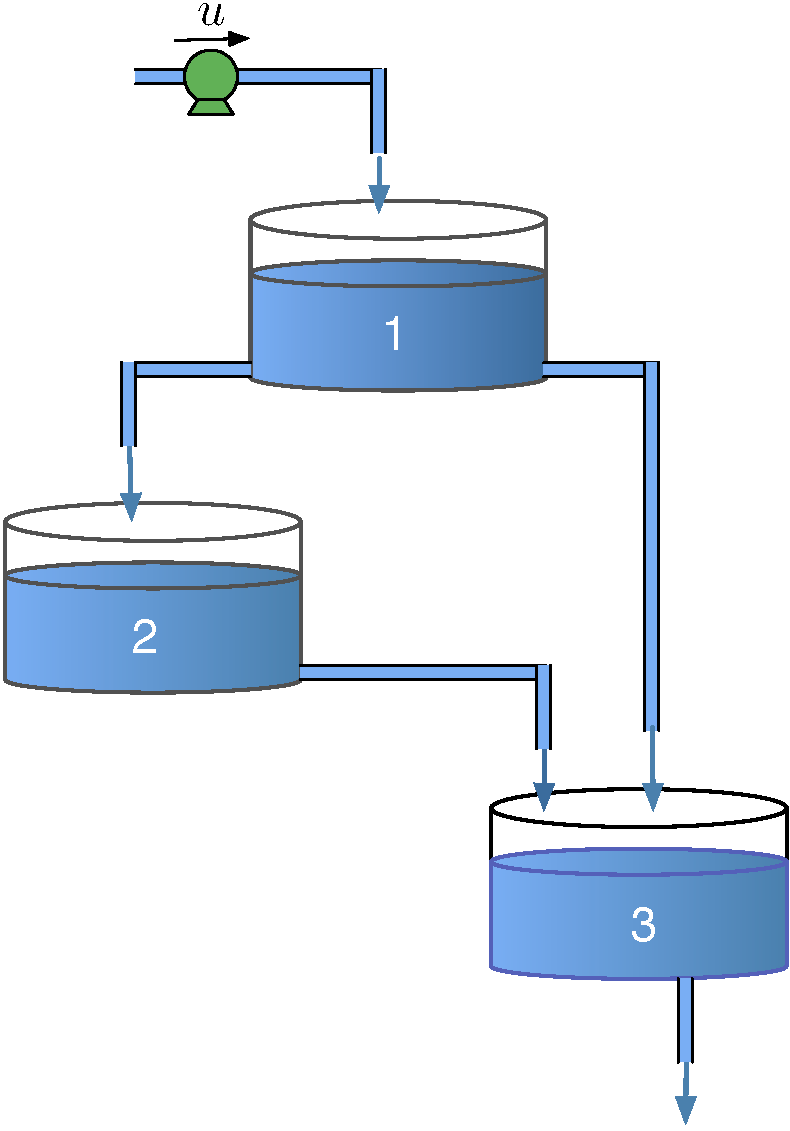
\includegraphics[width=7cm]{images/cascade}
\caption{Waterfall of tanks.}
\label{Fig:cascade}
\end{center} 
\end{figure}

It is clearly a compartment system whose the associated graph 
is depicted at figure \ref{Fig:grafassoc} and whose the continuity 
equations are written as~:
\begin{equation*} \begin{split} 
\dot x_1 &= q_{01} - q_{12} - q_{13} \\
\dot x_2 &=  q_{12} - q_{23} \\
\dot x_3 &= q_{13} + q_{23} - q_{30} 
\end{split} \end{equation*}
\begin{figure}[h] 
\begin{center}
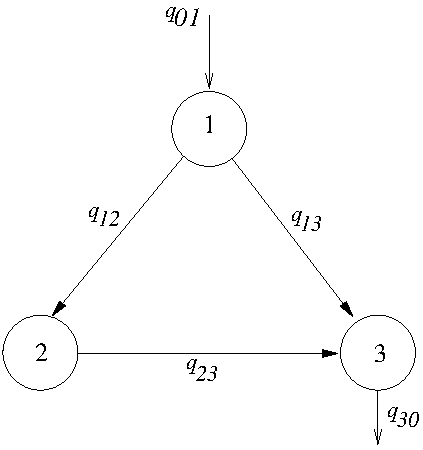
\includegraphics[width=7cm]{images/grafassoc}
\caption{Graph of the waterfall of tanks.}
\label{Fig:grafassoc}
\end{center} 
\end{figure}
In these equations, the sate variables $x_1$,$ x_2$ et $x_3$ specify, 
obviously, the volumes of water contained in the tanks; and the flows 
$q_{ij}$ depict the debits flowing from the upper tanks toward the lower 
tanks. In order to complete the model, the flows should be expressed in
terms of the sate variables and the input signals, correctly chosen.
The flow provided by the supply pomp of the upper tank can obviously be 
chosen as an input variable. The outgoing flow $q_{ij}$ of each tank 
is a positive function of the volume $x_i$ of the tank. The form of 
this function depends on the shape of the tanks and the configuration of 
the holes through which the water flows. Let's consider the case where the tanks 
have a constant horizontal section and where the flow goes through a 
rectangular hole located at the bottom of the tanks. The elevation of the water in 
a tank is expressed as~:
\eqnn
h_i = \frac {x_i}{S_i}
\eeqnn
where $S_{i}$ specifies the section of the tank.
According to the hydraulic laws, we know that when the elevation of the water $h_i$ is big 
toward the elevation of the hole, the link between the elevation of the water is proportional to 
$\sqrt{h_i}$ (Torricelli's law~\footnote{This law written by Torricelli in 1643 states that the speed $v$ of
the outgoing water of a tank of elevation $h$ verifies $v^2=2gh$. It can be proven intuitively by 
analogy with a body in free fall: a elementary volume of water at the surface of the tank has a potential energy 
$\rho g h$ and a kinetic energy $\rho v^2/2$ when it reaches the exit of the tank, where $\rho$ depicts the 
density. More rigorously, this can be deduced from Bernoulli's theorem without pressure loss or pump $p+\rho gz +\rho v^2/2 = \mathrm{constante}$, where $p$ depicts the pressure and $z$ the elevation.}). However, when the elevation of the water is lower than the elevation of the hole, the flows becomes proportional to $h_i\sqrt{h_i}$ 
(law of flows for a rectangular tank). A model of the following form can be given~:
\eqnn
q_{ij} = \frac { \alpha_{ij}h_i\sqrt{h_i} }{ \beta_{ij} + h_i}
\eeqnn
where $ \alpha_{ij}$ et $ \beta_{ij}$ are positive constants. Indeed, this model verifies the 
property telling that, for low water elevations ($h_i \ll \beta_{ij}$), the flow $q_{ij}$ is proportional to 
$h_i\sqrt{h_i}$ whereas for high water elevations ($h_i \gg \beta_{ij}$), the flow $q_{ij}$ is 
proportional to $\sqrt{h_i}$.
The flows $q_{ij}$ can be expressed in terms of $x_i$~:
\eqnn
q_{ij}(x_i) = \frac {k_{ij}x_i\sqrt{x_i} }{S_i \beta_{ij} + x_i} \hh \mbox{ avec } k_{ij} \triangleq \frac{\alpha_{ij}}{\sqrt{S_i}} 
\eeqnn
Finally, the state model can be written as~:
\begin{equation} \begin{split} \label{modetacasca}
\dot x_1 &= - \frac {k_{12}x_1\sqrt{x_1} }{S_1\beta_{12} + x_1} - \frac {k_{13}x_1\sqrt{x_1} }{S_1 \beta_{13} + x_1} + u, \\
\dot x_2 &=  \frac {k_{12}x_1\sqrt{x_1} }{S_1 \beta_{12} + x_1} - \frac {k_{23}x_2\sqrt{x_2} }{S_2 \beta_{23} + x_2},
\\
\dot x_3 &= \frac{k_{13}x_1\sqrt{x_1} }{S_1 \beta_{13} + x_1} + \frac {k_{23}x_2\sqrt{x_2} }{S_2 \beta_{23} + x_2} -
\frac {k_{30}x_3\sqrt{x_3} }{S_3 \beta_{30} + x_3}.
\end{split} \end{equation}
Let's notice that the functions $q_{ij}(x_{i})$ verifies the positivity conditions C1, C2 and C3. \qed
\end{exemple}

\section{Modèles linéaires avec commande par les alimentations 
extérieures}

C'est la classe de modèles à compartiments que l'on rencontre le plus
couramment dans la littérature. Elle est caractérisée par les définitions
suivantes des flux~:
\begin{enumerate}
\item Les flux entre compartiments et les flux de sortie du système sont 
des fonctions linéaires du
niveau du compartiment donneur :
\eqnn
q_{ij} = k_{ij}x_i \hspace{1cm} k_{ij} > 0 \hspace{1cm} (i=1,...,n;j=0,...,n)
\eeqnn
\item Les entrées $u_{\ell}$ du système sont proportionnelles aux flux
d'alimentation~: 
\eqnn
q_{0\ell} = k_{0\ell}u_{\ell} 
\eeqnn
\end{enumerate}
Dans ce cas, l'information nécessaire à l'écriture du modèle d'état 
est entièrement contenue dans le graphe du système. Le modèle d'état
prend la forme générale d'un système linéaire (voir chapitre 1), c-à-d~:
\eqnn
\dot{x} = Ax + Bu
\eeqnn
mais avec les particularités structurelles suivantes~:
\begin{enumerate}
\item La matrice $A$ est une {\em matrice de Metzler} c-à-d  telle que $a_{ij} 
\geq 0$ 
pour tout $i \neq j$
\item La matrice $A$ est diagonalement dominante c-à-d
\eqnn
|a_{ii}| \geq \sum_{j \neq i} a_{ji} 
\eeqnn
\item La matrice $B$ est une {\em matrice élémentaire} de plein rang, c'est à
dire une matrice qui contient au plus un élément non nul par ligne et par
colonne.
\end{enumerate}

\begin{exemple}

Le modèle d'état linéaire du système à compartiments
correspondant au graphe de la figure \ref{fig:exemplecomp} 
s'écrit comme suit~:
\begin{equation} \begin{split}
\bma{c} \dot x_1 \\ \dot x_2 \\ \dot x_3 \ema &= 
\bma{ccc} -(k_{12} + k_{13}) & k_{21} & 0 \\ 
k_{12} & -(k_{21} + k_{23}) & 0 \\ k_{13} & k_{23} & - k_{30} \ema
\bma{c} x_1 \\ x_2 \\ x_3 \ema \\ &\hd
+ \bma{cc} k_{01} & 0 \\ 0 & k_{02} \\ 0 & 0 \ema
\bma{c} u_1 \\ u_2 \ema
\end{split} \end{equation}
On observe que $A$ est bien une matrice de Metzler diagonalement
dominante et que $B$ est une matrice élémentaire de plein rang ($= 2$).
\cqfd
\end{exemple}

\begin{exemple}{\bf \em Modélisation physiologique}

Les physiologistes s'intéressent souvent à décrire et à analyser la 
propagation de substances biologiques ou chimiques dans le corps des
mammifères. Il peut s'agir de substances médicamenteuses (on parle alors
d'études pharmacocinétiques) ou encore de substances toxiques absorbées
volontairement ou accidentellement. Il peut s'agir aussi de substances d'origine
naturelle telle que des hormones ou des protéines. Les modèles à 
compartiments sont fréquemment utilisés pour procéder à de telles 
études : le corps du mammifère est alors représenté par un ensemble
plus ou moins diversifié de réservoirs interconnectés. 

Considérons l'exemple
de la figure \ref{Fig:grapharmaco}.
\begin{figure}[ht] 
\begin{center}
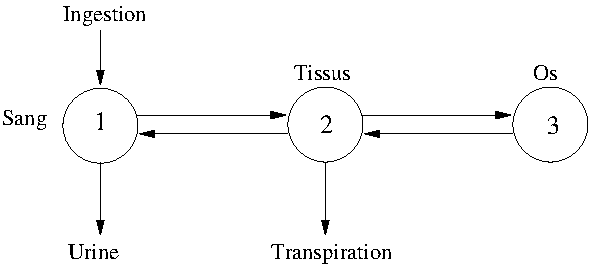
\includegraphics{images/grapharmaco}
\caption{Graphe d'un modèle à compartiments en pharmacocinétique}
\label{Fig:grapharmaco}
\end{center} 
\end{figure}
Une substance toxique (par exemple du plomb) est ingérée par un animal et
pénêtre dans le sang. Cette substance  se propage progressivement
dans le corps, passant du sang vers les tissus tout d'abord, vers les os ensuite.
Elle est excrétée par la transpiration d'une part et par les voies urinaires
d'autre part. Le modèle à compartiments linéaires correspondant
au graphe de la figure \ref{Fig:grapharmaco} est le suivant :
\begin{equation*} \begin{split}
\bma{c} \dot x_1 \\ \dot x_2 \\ \dot x_3 \ema &= 
\bma{ccc} -(k_{10} + k_{12}) & k_{21} & 0 \\ 
k_{12} & -(k_{20} + k_{21} + k_{23}) & k_{32} \\ 0 & k_{23} & - k_{32} \ema
\bma{c} x_1 \\ x_2 \\ x_3 \ema \\
& \hd + \bma{c} k_{ 01}\\ 0 \\ 0 \ema u.
\end{split} \end{equation*}
Dans ce modèle, les variables d'état $x_1$, $x_2$ et $x_3$ désignent
bien s\^ur les quantités de substance toxique dans les trois compartiments
(sang, tissus et os). La variable d'entrée $u$ désigne le flux d'ingestion 
par le corps.
\cqfd
\end{exemple}

\section{Modèles non linéaires avec commande par les flux}

Nous considérons maintenant des systèmes non linéaires à compartiments
dont les flux
$q_{ij}$ peuvent être des fonctions non linéaires quelconques de
leurs arguments satisfaisant les conditions C1 - C3. Nous avons déjà rencontré
un modèle non linéaire dans l'exemple de la cascade de
réservoirs. Toutefois, dans cet exemple, les flux entre 
compartiments n'étaient pas fonction des variables d'entrée $u_{\ell}$. Ici nous
considérerons le cas où certains flux entre compartiments sont des fonctions
explicites de variables d'entrée $u_{\ell}$ qui permettent de contr\^oler le débit
passant entre ces compartiments.  On utilise la représentation
symbolique de la figure
\ref{Fig:contflux} pour indiquer la présence d'une telle variable de contr\^ole.
\begin{figure}[ht] 
\begin{center}
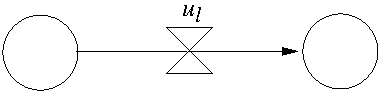
\includegraphics{images/contflux}
\caption{Représentation symbolique d'un flux contr\^olé}
\label{Fig:contflux}
\end{center} 
\end{figure}

\begin{exemple}{\bf \em Réseau de réservoirs}

Considérons le système hydraulique illustré à la figure \ref{Fig:reseauh}. Ce
réseau de réservoirs est celui de l'exemple de la cascade de
réservoirs (exemple \ref{systhyd}) que nous avons rencontré
précédemment, mais avec une petite modification~: l'écoulement entre le
réservoir $2$ et le réservoir $3$ n'est plus un écoulement libre mais est devenu
un écoulement forcé par la pompe. Dans la mesure où cette pompe est
commandable, il est naturel de considérer le débit pompé $F$ comme une variable
d'entrée. 

\begin{figure}[h] 
\begin{center}
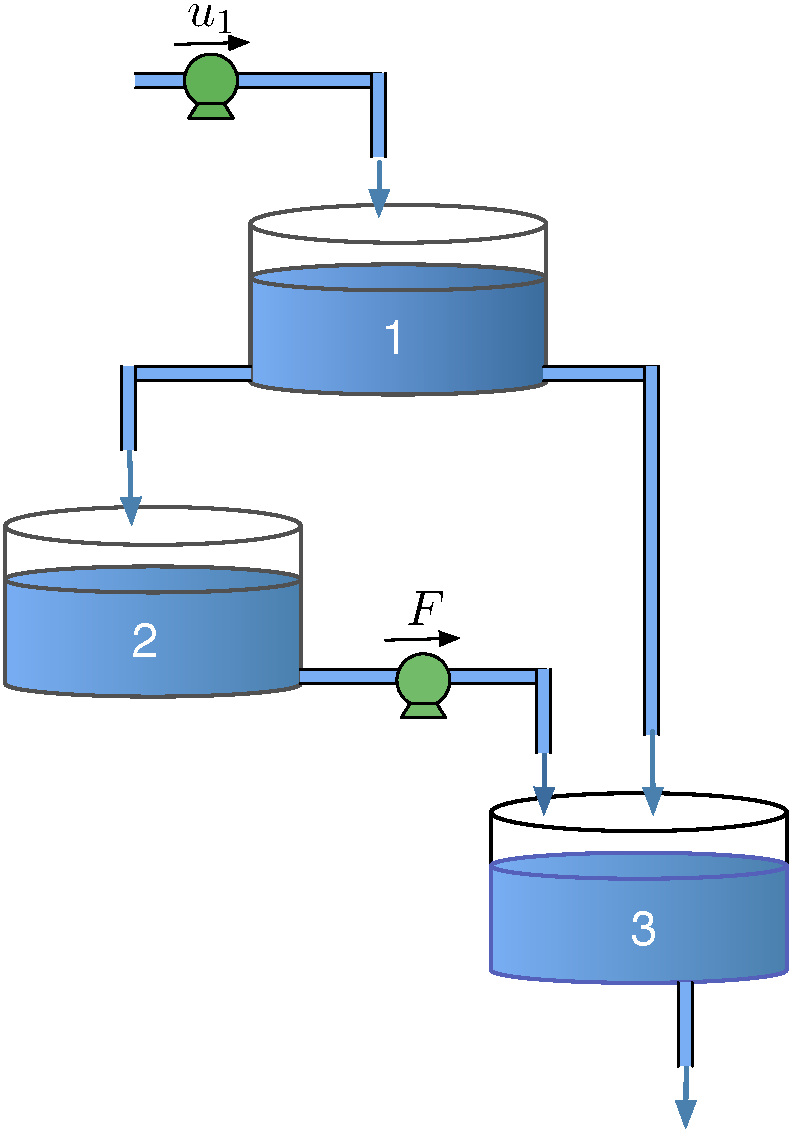
\includegraphics[width=7cm]{images/reseauh}
\caption{Réseau de réservoirs}
\label{Fig:reseauh}
\end{center} 
\end{figure}

Le modèle d'état (\ref{modetacasca}) que nous avions obtenu pour la cascade de
réservoirs est alors simplement modifié comme suit~:
\begin{equation} \begin{split}
\dot x_1 &= - q_{12}(x_1) - q_{13}(x_1) + u_1 \\
\dot x_2 &=  q_{12}(x_1) - u_2 \label{modres1} \\
\dot x_3 &= q_{13}(x_1) - q_{30}(x_3) + u_2 
\end{split} \end{equation}
où les variables d'état $x_i$ sont les volumes d'eau contenus dans les
réservoirs, la variable d'entrée $u_1$ est le débit d'alimentation du premier
réservoir, la variable d'entrée $u_2 = F$ est le débit pompé du deuxième 
vers le troisième  réservoir et les fonctions $q_{ij}(x_i)$ sont définies comme suit~:
\eqnn
q_{ij}(x_i) = \frac {k_{ij}x_i\sqrt{x_i} }{S_i \beta_{ij} + x_i}
\eeqnn
On observe que ce modèle d'état {\it ne peut pas} être celui d'un système à
compartiments vérifiant les conditions C1 - C3. En effet le flux $q_{23} = u_2$ ne vérifie pas la condition C3 et le système n'est pas positif : une simulation de ce modèle peut
conduire à des niveaux négatifs dans les réservoirs (même si les débits
pompés restent positifs) ce qui est évidemment contradictoire avec la réalité
physique. La difficulté provient du fait que, avec le modèle tel qu'il est écrit, on
peut pomper de l'eau dans le deuxième réservoir même quand il est vide !

On contourne aisément cette difficulté si on modélise le flux $q_{23}$ (qui est le
débit pompé $F$) de manière à respecter la réalité physique et à satisfaire la
condition C3 comme ceci~:
$$
q_{23}(x_2,u_2) = \phi(x_2)u_2
$$
où $\phi(x_2)$ est une fonction positive vérifiant $\phi(0) = 0$ et
$u_2$ représente l'actionnement de la pompe. On obtient alors un système à
compartiments dont le graphe est présenté à la figure \ref{Fig:graphreseau} et
dont le modèle d'état s'écrit~:
\begin{equation*} \begin{split}
\dot x_1 &= - q_{12}(x_1) - q_{13}(x_1) + u_1 \\
\dot x_2 &=  q_{12}(x_1) - \phi(x_2)u_2 \\
\dot x_3 &= q_{13}(x_1) - q_{30}(x_3) + \phi(x_{2})u_2 
\end{split} \end{equation*}
\begin{figure}[h] 
\begin{center}
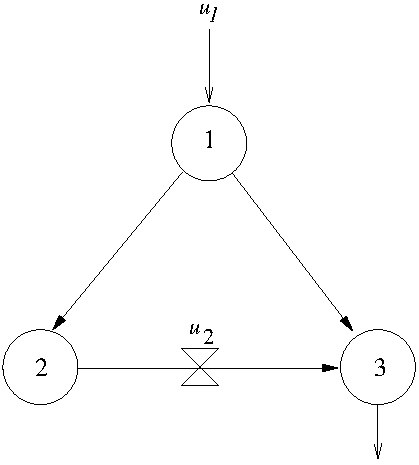
\includegraphics[width=7cm]{images/graphreseau}
\caption{Graphe associé au réseau de réservoirs}
\label{Fig:graphreseau}
\end{center} 
\end{figure}
\cqfd
\end{exemple}

La propriété structurelle fondamentale des systèmes linéaires à
compartiments se généralise aux systèmes non linéaires de la manière
suivante.
\begin{theoreme} 

Soit un système non linéaire à compartiments dont les flux $q_{ij}$ vérifient les
conditions C1 - C3. Alors les flux peuvent s'écrire de la fa\c con suivante~:
\eqnn
&& q_{ij}(x,u) = a_{ij}(x,u)x_i \hspace{4mm}
(i=1,...,n;j=1,...,n)\\ 
&& q_{i0}(x,u) = a_{i0}(x,u)x_i \hspace{4mm}
(i=1,...,n)\\
&& q_{0i} = k_{0i}u_i
\eeqnn
où les fonctions $a_{ij}(x,u)$ et $a_{i0}(x,u)$, définies sur
l'orthant positif, sont continues. 

En conséquence, le modèle d'état du système peut se mettre sous la forme
suivante~:
$$
\dot x = A(x,u)x + Bu
$$
où la matrice $A(x,u)$ est une matrice de Metzler diagonalement dominante pour
tout $(x,u)$ dans l'orthant positif et $B$ est une matrice élémentaire.
\cqfd
\end{theoreme}
Nous terminons ce chapitre par la présentation d'un autre exemple industriel
classique de système à compartiments.
\begin{exemple}{\bf \em Procédé de distillation binaire}

Un procédé de distillation binaire est un procédé utilisé pour séparer un
mélange de deux composés chimiques, sous forme liquide, appelé {\em charge}. Un {\it
dépropaniseur} ayant pour fonction de séparer le propane du butane est un
exemple typique de procédé de distillation binaire dans l'industrie pétrochimique.

La séparation s'effectue par évaporation dans une enceinte fermée appelée {\em ballon} (voir figure \ref{Fig:distillation}).
\begin{figure}[h]
\begin{center}
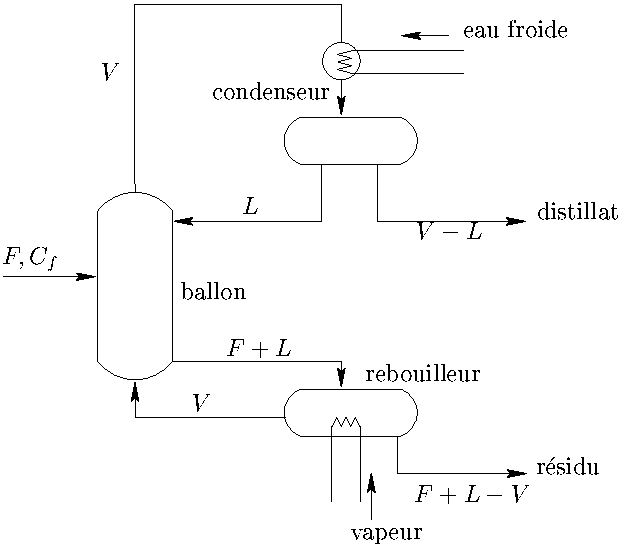
\includegraphics[width=8cm]{images/proc_distil}
\caption{Procédé de distillation}
\label{Fig:distillation}
\end{center} 
\end{figure}
Au sommet du ballon sort le {\it distillat} contenant essentiellement le composé léger avec
un peu de composé lourd. Au fond du ballon sort le {\it résidu} qui contient
essentiellement le composé lourd avec un peu de composé léger. Le ballon est alimenté par la charge avec un débit molaire $F$ (mol/min). Le flux de vapeur sortant au sommet du ballon est refroidi et complètement condensé. Le liquide
sortant du condenseur est partiellement recyclé vers le ballon avec un débit
molaire $L$. Le reste, appelé {\it distillat}, est extrait du système. En fond de
ballon, le liquide sortant est
réchauffé dans un rebouilleur et la vapeur ainsi produite est recyclée dans le ballon.  Le reste, appelé {\it résidu}, est extrait.

On présente ci-dessous un modèle simplifié de la dynamique de ce procédé de distillation en faisant les
hypothèses de modélisation suivantes~:
\begin{enumerate}
\item la charge est liquide et à sa température de bulle;
\item les phases liquide et vapeur dans le ballon et le rebouilleur sont homogènes et à
l'équilibre;
\item dans le ballon la pression est constante et il n'y a pas d'accumulation de vapeur; cette hypothèse permet d'omettre les dépendances en pression dans les équations et implique que le débit de vapeur $V$  à la sortie du ballon est égal au débit à l'entrée; 
\item les débits d'extraction liquide sont ajustés de manière que les masses molaires totales de la phase liquide dans les trois récipients soient constantes : le distillat est donc extrait avec un débit molaire $V-L$, le liquide en fond de ballon avec un débit molaire $F+L$ et le résidu avec un débit molaire $F+L-V$. Evidemment, cela implique que l'inégalité $0 < L < V < F+L$ soit vérifiée.\\
\end{enumerate}
Ainsi décrit, le procédé de distillation peut être vu comme un système à
compartiments dont le modèle dynamique est constitué des
équations de bilan de l'un des deux composés dans le ballon, dans le condenseur et dans le rebouilleur. Le graphe de ce système à
compartiments est présenté à la figure \ref{Fig:graphdisti} et les équations
d'état sont les suivantes~:
\begin{equation*} \begin{split}
\dot x_1 &= u_2 k(x_2) - u_{1}\frac{x_1}{m_1} - (u_2 - u_1) \frac{x_1}{m_1}\\
\dot x_2 &= u_1\frac{x_1}{m_1} - (u_1+u_3)\frac{x_2}{m_2} + u_2(k(x_3) - k(x_2)) + u_3c_f\\
\dot x_3 &= (u_1 + u_3)(\frac{x_2}{m_2} - \frac{x_3}{m_3}) + u_2(\frac{x_3}{m_3} - k(x_3))
\end{split} \end{equation*}
\begin{figure}[h]
\begin{center}
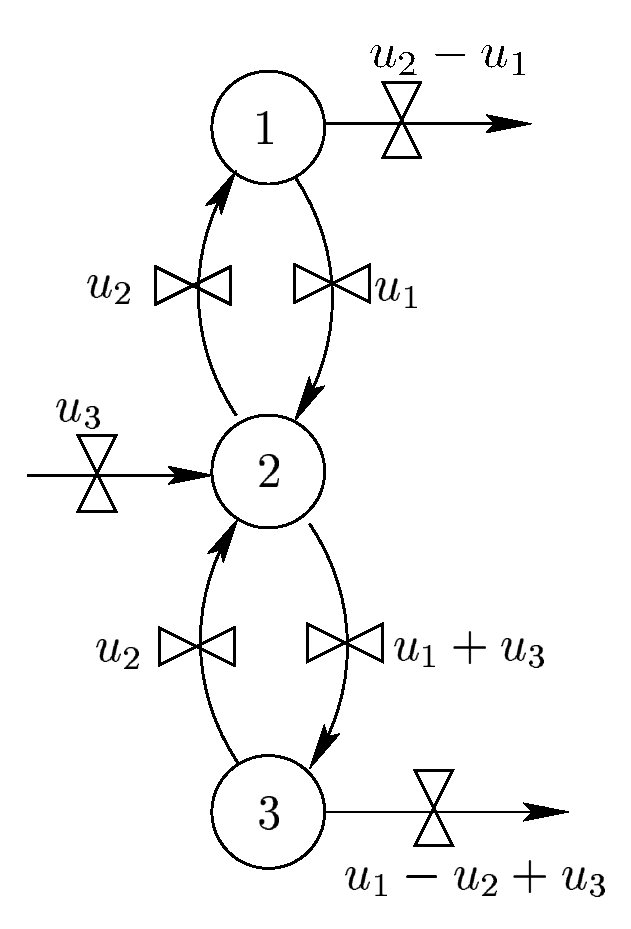
\includegraphics[width=5cm]{images/graphprocdistil}
\caption{Graphe associé au procédé de distillation}
\label{Fig:graphdisti}
\end{center} 
\end{figure}
Dans ces équations, les variables d'état $x_i$ représentent la masse molaire du
composant léger dans la phase liquide du condenseur (indice $1$), du ballon (indice $2$) et du rebouilleur (indice  $3$); les paramètres $m_i$ sont les 
masses molaires totales (et constantes) correspondantes : le rapport $x_i/m_i$ est la {\it fraction molaire}; le paramètre $c_f$
est la fraction molaire du composé léger dans la charge; les variables d'entrées $u_1 =
L$, $u_2 = V$ et
$u_3 = F$ sont, respectivement, les débits molaires de reflux, de production de vapeur et
d'alimentation. Enfin, la fonction $k(x)$ est une relation d'équilibre
liquide-vapeur permettant de relier la fraction molaire du composant léger quittant le liquide
sous forme vapeur à la fraction molaire du composant dans la phase liquide. 
\begin{figure}[ht]
\begin{center}
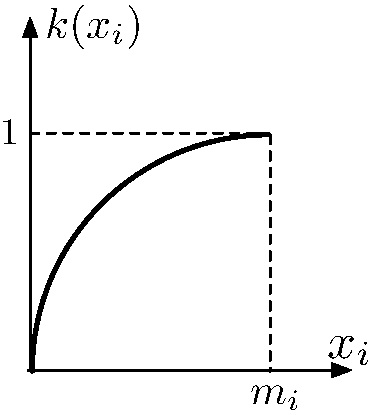
\includegraphics[width=4cm]{images/separ}
\caption{Relation d'équilibre liquide-vapeur}
\label{Fig:separ}
\end{center} 
\end{figure}

\noindent Cette
relation s'exprime classiquement comme suit~:
\eqnn
k(x_i) \triangleq \frac{\alpha x_i}{m_i + (\alpha - 1)x_i}
\eeqnn
où le paramètre constant $\alpha > 1$ porte le nom de facteur de séparation.
Cette fonction, définie sur l'intervalle $[0,m_i]$, vérifie $k(0) = 0$ et
$k(m_i) = 1$ (voir figure \ref{Fig:separ}). \qed  
\end{exemple}

\section{Exercices}

\begin{exercice}{\bf \em Un système à compartiments}

Soit le système dynamique suivant:
\begin{align*}
\dot x_{1} &= x_{3} - \log (1+x_{1}) \\
\dot x_{2} &= x_{3} - x_{2}^2 \\
\dot x_{3} &= x_{2}^2 - 2x_{3} + u
\end{align*}
Démontrer qu'il s'agit d'un système à compartiments. Dessiner le graphe associé. Calculer les flux $q_{ij}$, la matrice $L$ et la matrice $A(x,u)$. \qed
\end{exercice}
\vv

\begin{exercice}{\bf \em Un système hydraulique}

Un système hydraulique comportant trois réservoirs et deux pompes
est représenté à la figure \ref{Fig:systhydr}.
\begin{figure}[h]
\begin{center}
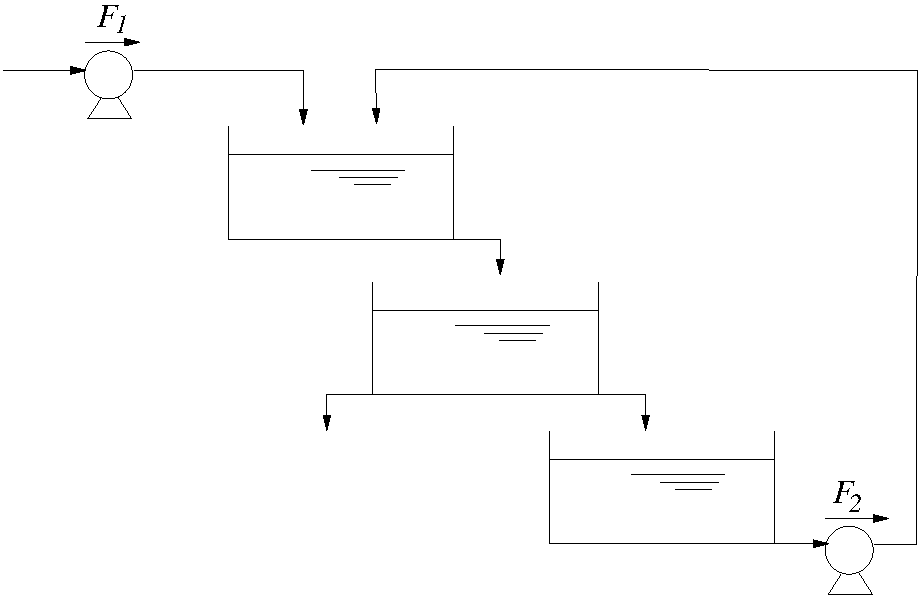
\includegraphics[width=8cm]{images/systhydr}
\caption{Système hydraulique}
\label{Fig:systhydr}
\end{center} 
\end{figure}
\begin{enumerate}
\item Etablir un modèle d'état du système en considérant les
débits volumétriques $u_1 = F_1$ et $u_2 = F_2$ comme variables
d'entrée. Montrer que le système obtenu n'est {\it pas} un système
positif. 
\item Proposer une autre définition de la variable d'entrée $u_2$ qui
garantisse que le système soit positif. 
\item Dessiner le graphe du modèle à compartiments ainsi obtenu. \qed
\end{enumerate}
\end{exercice}
\vv 

\begin{figure}[!ht] 
\begin{center}
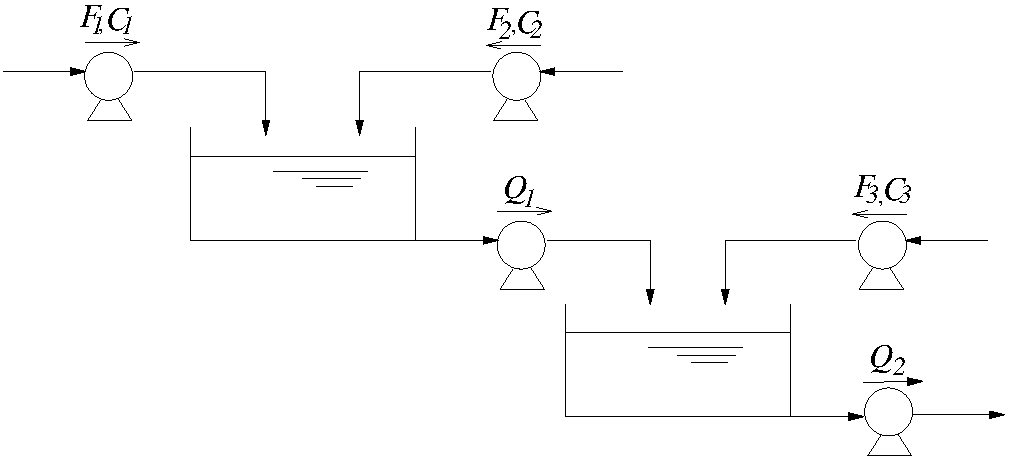
\includegraphics[width=8cm]{images/cuvmel}
\caption{Réseau de cuves de mélange}
\label{Fig:cuvmel}
\end{center} 
\end{figure}

\begin{exercice}{\bf \em Un réseau de cuves de mélange}

Le système représenté à la figure \ref{Fig:cuvmel} est con\c cu pour
mélanger trois substances $X_1, X_2, X_3$ dont les concentrations
d'alimentation sont notées $C_1, C_2, C_3$. Les volumes contenus
dans les deux cuves sont notés $V_1, V_2$. Les débits volumétriques
des pompes sont notés $Q_1, Q_2, F_1, F_2, F_3$.

\begin{enumerate}
\item Etablir un modèle d'état du système avec les variables
d'entrée suivantes~: $u_1 = Q_1/V_1, u_2 = Q_2/V_2, u_3 = C_1, u_4 =
C_2, u_5 = C_3$. Les débits $F_i$, $i = 1, \dots , 3$, sont supposés
constants.
\item Justifier la forme des variables d'entrées $u_1$ et $u_2$. \qed
\end{enumerate}
\end{exercice}
\vv

\begin{exercice}{\bf \em Modèle linéaire à compartiments}

Caractériser la structure du graphe d'un modèle linéaire à
compartiments dont la matrice $A$ est~:
\begin{enumerate}
\item bidiagonale
\item tridiagonale
\item triangulaire inférieure \qed
\end{enumerate}
\end{exercice}
\vv

\begin{exercice}{\bf \em Modèle du  procédé de distillation}

Déterminer la matrice $A(x,u)$ du modèle du procédé de distillation. \qed
\end{exercice}
\vv

\begin{exercice}{\bf \em Des réservoirs communicants}

Un système à deux réservoirs communicants est représenté à la
figure \ref{Fig:reservoircom} Le liquide s'écoule librement entre les deux
réservoirs et vers l'extérieur sous l'action de la pression hydrostatique.

\begin{figure}[h]
\begin{center}
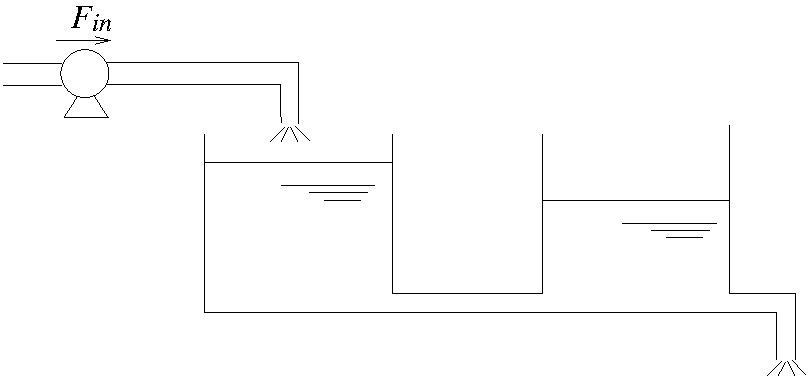
\includegraphics[width=8cm]{images/reservoircom}
\caption{Réservoirs communicants}
\label{Fig:reservoircom}
\end{center} 
\end{figure}

\begin{enumerate}
\item Etablir un modèle d'état du système. Le débit fourni par la
pompe d'alimentation est la seule variable d'entrée du système.
\item Montrer qu'il s'agit d'un système à compartiments. Dessiner le
graphe associé. Expliciter les flux entre compartiments. \qed
\end{enumerate}
\end{exercice}


\end{document}
